\section{design document}
\subsection{Purpose}
The problem we are trying to solve is how to map a RESTful API onto a POSIX filespace. This allows users to browse the data in a familiar topography and also utilize various command-line tools for browsing, manipulating, creating, and deleting data. 

Our program is meant to be used by an average user who has a basic understanding of file systems and command-line tools. Our goal is to abstract the process so that the user does not need to know the specific RESTful API, he or she simply needs to know simple file operations in order to interact with the program.

\subsection{High Level Entities}
Our design consists of a RESTful API that interfaces with our ruby program. For demonstration purposes we are basing our implementation off of the Twitter API(\textit{http://http://dev.twitter.com/doc})The Ruby middleware uses Sinatra for pairing methods with RESTful routes. We use the ruby implementation of the FUSE (Fileystem in User SpacE) (\textit{https://rubyforge.org/projects/fusefs/}) to actually mimic a POSIX filesystem on the user's local environment. All data will be fetched from the API. We may implement a caching algorithm if time allows, but the program should be designed to allow caching to be implemented.   

\subsection{Top Level Archetecture}

\subsubsection{Processing Elements}

\paragraph{The FUSE driver} handles file system requests generated due
to user actions on particular file paths as described in the requirements
document. It converts these requests into an http request which is forwared to
the Sinatra backend.

\paragraph{The Router} implements a simple http web server which listens to requests from
the FUSE driver. This will be implemented using the Sinatra framework, which
will match against a requested uri and invoke a specific handler. These handlers
will be responsible for fetching/manipulating the twitter data via the
webservice api provided by twitter.

\paragraph{Twitter API} will be leveraged to actually interact with the data as
requested by the user.

\subsection{Connecting Elements}

The above processing elements are connected to form a layered architecture as
shown in figure~\ref{fig:top-top} below.

\begin{figure}[h]
\centering
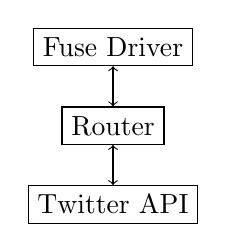
\begin{tikzpicture}
  \node [draw] at (0,0)    (Bottom) {Twitter API};
  \node [draw] at (0,1)    (Middle) {Router};
  \node [draw] at (0,2)    (Top)    {Fuse Driver};

  \draw [<->] (Bottom) -- (Middle);
  \draw [<->] (Middle) -- (Top);
\end{tikzpicture}
\caption{Top Level Components.}\label{fig:top-top}
\end{figure}

